%----------------------------------------------------------------------------
\chapter{Test Framework} \label{test-framework}
%----------------------------------------------------------------------------

This chapter presents the design and implementation of the test framework that facilitates the automatic deployment of the sample application and running the measurements to determine the dependability metrics of the system.

%----------------------------------------------------------------------------
\section{Introduction}
%----------------------------------------------------------------------------

Now, that the sample application is ready, it is time to examine its robustness. The goals of the thesis project included measuring the dependability of the sample application with optional fault injection to simulate possible real-world anomalies. The following sections present the aspects of the design and the construction of a framework that enables collecting dependability metrics and injecting failure scenarios into the sample application (see Section \ref{test-framework-design}). As a result these considerations, a test framework was created using various technologies (Python, Chaos Mesh, Prometheus, Jenkins, etc.) that can be used to conduct highly configurable and reproducible dependability analyses of the sample application. The implementation of the framework is discussed in details in Section \ref{test-framework-impl}. The created framework was then used to execute initial measurements determining the characteristics of the system in its original state (see Section \ref{baseline-results}).

%\begin{itemize}
%	\item what do we want? - measure the dependability of the application and inject faults into the system in an automated way
%	\item what are the goals?
%	\item lets create a framework - design and implement a tool that enables to constantly monitor the state of the system under test, collect dependability metrics and introduce different kinds of anomalies into the system
%	\item try it out - baseline measurements
%\end{itemize}

%----------------------------------------------------------------------------
\section{Design} \label{test-framework-design}
%----------------------------------------------------------------------------

Consistency is essential when testing. In order to get meaningful results that can be later used to evaluate the implementation and to draw conclusions, a well defined framework is needed that sets clear boundaries on how the results are acquired. The quality of the testing and measurement greatly depends on the way these activities are executed, which means that a detailed design of the framework is vital.

%\begin{itemize}
%	\item why is a framework needed
%	\item test framework architecture
%	\item what is the test objective?
%	\item what to test? - dependability metrics! - which ones?, how?
%	\item need to monitor the application metrics, state --> need for monitoring system
%	
%	\item how does running tests affect the result
%\end{itemize}

%----------------------------------------------------------------------------
\subsection{Test objective} \label{test-design-objective}
%----------------------------------------------------------------------------

The first thing to specify when designing a test framework is the test objective. This highly affects the way the framework should be planned and created.

The goal of the framework is to measure the dependability metrics of the sample application to reveal weak spots and to discover opportunities to improve the dependability of the application. The results of the measurements can be used later as reference values when introducing various kinds of enhancements to the system to make the metrics better. The enhancements are described in Chapter \ref{enhancements}.

%----------------------------------------------------------------------------
\subsection{Requirements} \label{test-design-req}
%----------------------------------------------------------------------------

The design of the test framework was driven by several requirements to create an architecture that facilitates achieving the test objective defined in the previous section.

\paragraph{Configurable} In order to support various kinds of test scenarios, the framework should be highly configurable. This characteristic also makes the testing system more reusable and generic, so it is not closely tailored to the sample application described in this project.

\paragraph{Reproducible} The framework should function in a fairly deterministic way. This means that any two test executions with the same configuration should produce approximately the same results. As the applications that the framework is designed to evaluate are Kubernetes based, distributed systems, requiring complete deterministic behavior of the framework is not realistic. There are several things that can introduce a slight level of randomness to the application. For example the state of the network between the components or the way the fault injection logic inserts anomalies into the system (further details in section \ref{test-design-fault-injector}).

\paragraph{Automated} The usability of the framework greatly depends on how much manual interaction is needed for it produce results. Ideally, the framework should not require any human actions to be able to function after the configurations are correctly set. Automation enables the users of the framework to define multiple test scenarios with different configurations, collect them into a script and start all the measurements with only one command. Furthermore, if the framework is able to operate autonomously once it gets the right inputs, it can be integrated into existing pipelines (Continuous Integration, Continuous Delivery) to act as a quality gateway before an application is deployed into production.

%\begin{itemize}
%	\item Reproducible
%	\item Automated
%	\item Configurable
%\end{itemize}

%----------------------------------------------------------------------------
\subsection{Framework workflow} \label{test-design-workflow}
%----------------------------------------------------------------------------

%	\item Introduce abstract workflow \begin{enumerate}
%		\item Prepare infrastructure and application
%		\item Generate load
%		\item Inject faults
%		\item Collect metrics -  need to monitor the application metrics, state --> need for monitoring system
%		\item Store results
%	\end{enumerate}


Considering the test objective and the requirements described in the previous sections, the functional workflow of the testing framework can be seen in Figure \ref{fig:test_framework_workflow}.

\begin{figure}[h]
	\centering
	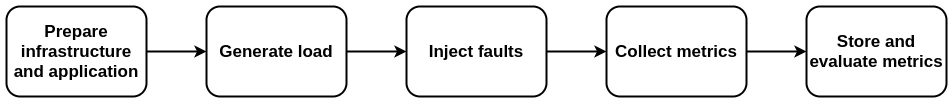
\includegraphics[width=140mm, keepaspectratio]{figures/test_framework_workflow.png}
	\caption{Test framework workflow}
	\label{fig:test_framework_workflow}
\end{figure}

As per this design, the framework should first prepare the environment for testing. This consists of setting up the Kubernetes infrastructure that the application will run on and starting the deployed application in this environment. After the application is running, in order to trigger to trigger task executions, a subsystem generates and sends load to the application. To better understand how the system under test behaves, different kinds of faults and anomalies are introduced to the system while the executions and possibly the load generation are in progress. The framework constantly collects the exposed metrics from the application and the infrastructure to gain insights about how the system manages to handle the implanted anomalies. After the load generation and the task executions are done, the metrics get stored and evaluated.

%----------------------------------------------------------------------------
\subsection{Architecture}
%----------------------------------------------------------------------------

The architecture of the test framework that facilitates the previously defined workflow is displayed in Figure \ref{fig:test_framework_arch}.

\begin{figure}[h]
	\centering
	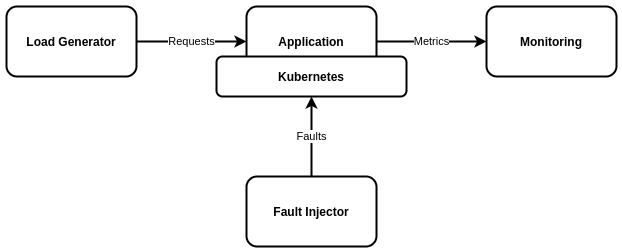
\includegraphics[width=140mm, keepaspectratio]{figures/test_framework_arch.png}
	\caption{Test framework architecture}
	\label{fig:test_framework_arch}
\end{figure}

The framework consists of three main components: the load generator, the fault injector and the monitoring subsystem. Each is described in the following sections.


%\begin{itemize}
%	\item architecture DIAGRAM
%	\item describe what each component does
%\end{itemize}


%----------------------------------------------------------------------------
\subsection{Load Generator}
%----------------------------------------------------------------------------

%\begin{itemize}
%	\item send HTTP requests to the backend according to pattern (uniform distribution)
%\end{itemize}

The responsibility of the load generator component is to simulate real world workload on the sample application. This way the framework can better assess the actual dependability characteristics of the system.

As the sample application (more precisely the backend) accepts user inputs in the form of HTTP requests, the load generator component should be able to produce correctly built up HTTP requests and send them to the application. This will trigger task executions and multiple worker instance deployments in case the requests are sent more frequently than a single worker could execute them one by one without leaving any tasks waiting in the message queue.

%----------------------------------------------------------------------------
\subsubsection{Parameters}
%----------------------------------------------------------------------------

% input value
% wait time between requests - different distributions
% number of simulated users

There are several ways to customize the way that load generation happens and how much workload it causes to the system under test.

\paragraph{Task input value} Probably the most trivial way is to change the task input value in the requests. As described in section \ref{impl-backend-interfaces}, the \texttt{input} field in the request JSON determines which Fibonacci number is calculated by a worker component. This means the time a worker instance spends on executing a task can be manipulated by the input value.

\paragraph{Request frequency} Another method that the load generator can exploit to control the workload on the system is to wait different amounts of time between sending individual requests. This can also model how real users would use the application. The wait time between requests can be a constant value, but in fact, it can be calculated based upon any arbitrary logic. Generally, various kinds of distribution functions are used to determine the request frequency.

\paragraph{Parallelism} To increase the workload on the system, multiple requests can be sent by the load generator in parallel. Using this together with increasing the request frequency can greatly intensify the load on the application. Similarly to the request frequency, the amount of requests to send in parallel can be calculated using any logic.


%----------------------------------------------------------------------------
\subsection{Fault Injector} \label{test-design-fault-injector}
%----------------------------------------------------------------------------

%\begin{itemize}
%	\item inject faults on different levels (Pod, Network, CPU, Memory)
%	\item periodic fault injection
%\end{itemize}

The aim of the fault injector component is to introduce different kinds of failure anomalies to the application in order to trigger fault tolerant mechanisms in the system if they exist.

The amount of possible failure anomalies proportionally increases with the complexity of the system and is most likely to be close to practically countless variations. To achieve the best results while limiting the number of failure anomalies to test, only the most common failure scenarios should be taken into account. Considering also the probability of the failure anomalies and applying only those to the system can result in a fairly good approximation of real world failure scenarios.

The following sections attempt to collect some of the most common anomalies that can cause errors or even outages in cloud based systems.

%----------------------------------------------------------------------------
\subsubsection{General failure anomalies}
%----------------------------------------------------------------------------

\paragraph{Network anomalies} Network anomalies include latency, jitter, slow bandwith, network partition. All of these can affect the performance and dependability of an application.

\paragraph{CPU starvation} CPU starvation can occur if there are multiple software components deployed to the same physical machine which is the case most of the time when using the products of cloud provider companies to run an application. If a process on a machine executes a CPU heavy computation, it can reserve most of the CPU capacity of the machine, leaving other processes without enough processor time which can cause transient or even permanent application failures.

\paragraph{Memory starvation} Memory starvation is similar to CPU starvation, only instead of sharing a machine with CPU usage heavy processes, there are programs that take up most of the memory of the physical machine.

\paragraph{Disk anomalies} Disk anomalies are probably the most common failure anomalies as these type of devices are used in enormous amounts in every data center. This class of anomalies can frequently occur in several different forms, for example disk I/O latency, read/write errors or complete device failures.

%----------------------------------------------------------------------------
\subsubsection{Kubernetes failure anomalies}
%----------------------------------------------------------------------------

As the target platform is Kubernetes, the final list of applicable failure scenarios should include Kubernetes related anomalies as well. Some possible examples are listed below.

\paragraph{Pod failure} Pod failures can happen for example in case of configuration errors or application errors. Typically, when a pod fails, it gets restarted by a \texttt{ReplicaSet} that may solve transient errors.

\paragraph{Pod death} Pods can be terminated due to human operational faults but also when the Kubernetes control plane decides to reschedule a pod to a different physical machine.

\paragraph{Cloud provider anomalies} Although Kubernetes clusters can be set up on private machines as well, generally they are used as a service offered by a cloud provider company. These products are highly available and are managed by experts, however, occasional errors can possibly happen in these type of environments too.

%----------------------------------------------------------------------------
\subsection{Monitoring} \label{test-design-monitoring}
%----------------------------------------------------------------------------
%need to monitor the application metrics, state --> need for monitoring system
% which metrics to collect
% whicch dependability metrics to use
% timeseries metrics
% vizualisation capabilities

The framework should be able to collect metrics about the infrastructure and the sample application. This requires that the framework should have a separate monitoring subsystem.

As the value of different metrics changes over time while the system executes task and while various failure anomalies are injected, the monitoring system should be able to handle time series data format effectively.

In order to increase the human usability of the framework, it is required that the monitoring system provides a visual interface where its users can track the status of the system under test during execution and to evaluate results.

There are a lot of metrics that the monitoring system can collect. Apart from the application specific custom metric like \texttt{worker\_busy\_thread} introduced in section \ref{impl-worker-custom-metrics}, Kubernetes itself exposes a vast amount of metrics in several categories. As the focus of the thesis is on measuring the dependability metrics, only the values related to this should be collected and used. Section \ref{background-dep-metrics-mean-values} and \ref{background-dep-metrics-prob-funcs} describes the possible dependability metrics that can be measured. The monitoring system targets collecting measurements for the following dependability metrics:

\begin{itemize}
	\item Mean Up Time
	\item Mean Down Time
	\item Mean Time Between Failures
	\item Availability
\end{itemize}

These metrics were chosen because they acceptably describe the dependability characteristics of a cloud based system that is designed to function continuously. 

%----------------------------------------------------------------------------
\section{Implementation} \label{test-framework-impl}
%----------------------------------------------------------------------------

%\begin{itemize}
%	\item Test environment locally or in cloud
%	\item how does running tests affect the 
%\end{itemize}

This section describes the implementation of the test framework and presents the decisions behind them.

Before going into the details of each subsystem in the framework, the environment of the test framework should be specified. The question is, where to run the framework? Should it be deployed next to the system under test to minimize communication overhead or should it run independently from the application?

Operating the test framework in the same environment as the tested application seems obvious at first, however this would bring in several issues that should be taken into account. Deploying the framework and the system under test would create a tightly coupled structure, whereas in distributed systems, loosely-coupled units are preferred. Co-deployment would also lead to the possibility that operating the framework could have a performance impact on the tested application itself, causing altered measurement results. Any infrastructural error (for example physical machine crash) -- either provoked by transient failures or inserted by the fault injector -- would affect both the application under test (which is accepted and should be handled by the application) and the framework itself. This is not passable as it would lead to framework malfunctions.

The conclusion is to deploy the test framework and the application to be evaluated separately. As it is practical for some of the tools used in the framework to run in the same Kubernetes cluster as the application, separation is implemented with exploiting two Kubernetes features. First, the framework is logically separated from the application by deploying them into different namespaces. Additionally, the two parts are physically separated as well using NodeSelectors in the Pod definitions of the components (for further information on NodeSelectors, see \cite{KubernetesNodeSelector}). This will ensure, that if a node that runs application workload is injected with machine failures, it will not have an effect on the test framework.

%----------------------------------------------------------------------------
\subsection{Measurement Proxy}
%----------------------------------------------------------------------------

The test framework requires a stable connection into the Kubernetes cluster in order to interact with the application. This is necessary for example to be able to generate load for the backend component. The evident solution for this would be to use the port-forwarding capabilities of the \texttt{kubectl} command line tool, that enables accessing application in a Kubernetes cluster from outside. However, as the application will be exposed to various kinds of failure scenarios by the fault injection subsystem, the connection to the backend component may be disrupted which presents complications to the framework.

Introducing a separate component to act as an entrypoint could provide a stable connection towards the application and support easier error handling due to lost connection to the backend. This extra unit -- called Measurement Proxy -- is an Nginx reverse proxy under the hood, that forwards all connection it receives to the backend component. This way, the test framework can use \texttt{kubectl} port-forwarding to connect to the Measurement Proxy and thus to the backend. The connection will not have to be renewed due to backend failures while the test framework will be notified of the error by the responses from the Measurement Proxy. The architectural place of the Measurement Proxy can be seen in Figure \ref{fig:measurement_proxy}.

To ensure that the Measurement Proxy is not affected by any of the injected fault scenarios, it must be separated from the application. This is accomplished by deploying the Measurement Proxy in a separate namespace (\texttt{measurement-proxy}) as the one that holds the application (\texttt{kubedepend}).

%\begin{itemize}
%	\item why is it needed - to ensure that the framework can always reach the app (pod kill can disrupt port-forwarding the backend service)
%	\item none of the fault injection cases affect the measurement proxy
%\end{itemize}

\begin{figure}[h]
	\centering
	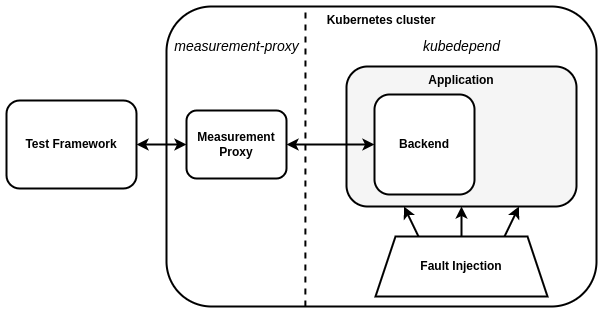
\includegraphics[width=140mm, keepaspectratio]{figures/measurement_proxy.png}
	\caption{The role of the Measurement Proxy}
	\label{fig:measurement_proxy}
\end{figure}

%----------------------------------------------------------------------------
\subsection{Kubedepend}
%----------------------------------------------------------------------------

%\begin{itemize}
%	\item what it is used for?
%	\item facilitates automatic load generation, fault injection, collecting results
%	\item describe its workflow
%	\item purpose of waiting for stable system state
%	\item prometheus metrics
%	\item parameters (click)
%\end{itemize}

Section \ref{test-design-req} emphasized the importance that the framework should be configurable, give reproducible results and be automated. To satisfy these requirements, a command line program in Python was created to enforce them as well as to implement the major part of the test framework workflow proposed in Section \ref{test-design-workflow}. This tool is named Kubedepend.

%----------------------------------------------------------------------------
\subsubsection{Configuration}
%----------------------------------------------------------------------------

Kubedepend supports easy configuration through exposing command line parameters that can be used to customize some behaviors of the tool.

This functionality is implemented with the help of the Click Python package \cite{Click}. Click enables creating clean command line interfaces in a composable way with as little code as necessary.

For instance, the user can specify the duration of the load generation, the types of failures anomalies to inject into the system and the number of tests to execute in sequence with the same configuration. The main configuration options are presented in later sections describing the implementation of the test framework workflow steps.

An example on how to define a command line parameter for the entrypoint of the Python program can be seen below.

\vspace{0.5cm}
\begin{minipage}{\linewidth}
	\begin{lstlisting}[language=python, caption={Define a parameter to control saving test results (simplified extract)}, label={lst:click-option}]
	@click.command()
	@click.option('--nosave', is_flag=True)
	def main(nosave):
		...
	
		click.echo('nosave=' + str(nosave))
		
		...\end{lstlisting}
\end{minipage}

%----------------------------------------------------------------------------
\subsubsection{Reproducibility}
%----------------------------------------------------------------------------

Kubedepend supports reproducible results in sense that when it is started with the same inputs, it executes the same logic to test and evaluate the system. 

%----------------------------------------------------------------------------
\subsubsection{Automation}
%----------------------------------------------------------------------------

After providing it with the right inputs, Kubedepend facilitates automatic load generation, fault injection and metric collection with the help of other third party tools later discussed in this chapter. When it is started, it is assumed that the Kubernetes infrastructure and the application are already ready and deployed. This means that it practically manages all the steps in Figure \ref{fig:test_framework_workflow} except the first one -- Prepare infrastructure and application. This step is executed by another mechanism that is later discussed (see Section \ref{cicd}).

%----------------------------------------------------------------------------
\subsubsection{Measurement and Measurement sequence} \label{test-impl-measurement-seq}
%----------------------------------------------------------------------------

In Kubedepend a Measurement represents the process of load generation, fault injection and metric collection. Section \ref{test-design-req} pointed out that it is not feasible to require completely deterministic results from the test framework. However, to even out the transient, temporary behaviors of the system, Kubedepend introduces the concept of Measurement Sequences. A Measurement Sequence is the collection of arbitrary number of individual Measurements with the same configuration. A single execution of Kubedepend carries out the running of one Measurement Sequence. The result of the Measurement Sequence is the collection of individual Measurement results. A graphical representation of the idea of Measurement Sequence can be seen in Figure \ref{fig:measurement_sequence}.

\begin{figure}[h]
	\centering
	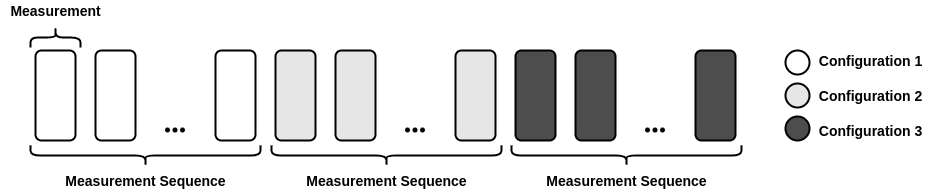
\includegraphics[width=140mm, keepaspectratio]{figures/measurement_sequence.png}
	\caption{Measurement Sequence}
	\label{fig:measurement_sequence}
\end{figure}

The number of Measurements to execute during a Measurement Sequence is set by an adaptive algorithm. After each Measurement, the results are evaluated and the standard deviation of the availability metric is calculated. A Measurement is re-executed with the same configuration until this value is less than or equal to a target value. The target value, the minimum and the maximum number of Measurements to run can be configured with parameters of Kubedepend (\texttt{target-std}, \texttt{min-measurement-count}, \texttt{max-measurement-count}). This mechanism attempts to lift the burden of fine-tuning the number of Measurements in case of each different scenario and to seek consistency in the results.

% TODO diagram about how Kubedepent connects to the different parts in the framework and the application

% wait for stable state -- why it is needed?

% the role of scheduled chaos experiment

\paragraph{Periodic Fault Injection} During a single Measurement Kubedepend injects failure anomalies periodically. This supports testing the robustness of the system under test and that how well the application can recover from failures.

\paragraph{Stable System State} Executing Measurement Sequences instead of a single Measurement introduces another complication to the test framework. It has to ensured that the effects of a previous Measurement does not have an impact on consequent Measurements. For this purpose, Kubedepend uses the notion of Stable System State which represents the state of the application under test, where all the components are up and running, there are no task executions in progress and there are not any messages waiting in the message queue. A Measurement can only be started if the application is in Stable System State.

%----------------------------------------------------------------------------
\subsubsection{Output} \label{test-impl-kubedepend-output}
%----------------------------------------------------------------------------
% what is the output data, what are the fields

Kubedepend saves the results of the measurements in a CSV file, where each row describes a Measurement in a Measurement Sequence. The CSV file has the following fields:

\begin{itemize}
	\item \texttt{id} - A unique identifier attached to the Measurement Sequence.
	\item \texttt{measurement\_seq\_start\_time} - The time when the Measurement Sequence was started.
	\item \texttt{availability} - The availability result of the application in a given Measurement.
	\item \texttt{mut} - The mean up time result of the application in a given Measurement.
	\item \texttt{mdt} - The mean down time result of the application in a given Measurement.
	\item \texttt{mtbf} - The mean time between failures result of the application in a given Measurement.
	\item \texttt{measurement\_start\_time} - The time when the given Measurement was started inside the Measurement Sequence.
	\item \texttt{measurement\_end\_time} - The time when the given Measurement ended inside the Measurement Sequence.
	\item \texttt{submitted\_jobs} - The number of jobs submitted by the client during a given Measurement.
	\item \texttt{finished\_jobs} - The number of successfully finished jobs during a given Measurement.
	\item \texttt{fault\_profile} - The fault profile used for fault injection during the Measurement Sequence.
	\item \texttt{cluster\_type} - The type of the Kubernetes cluster the application runs on. Can be set with the \texttt{cluster-type} Kubedend command line parameter. Possible values at the moment are \texttt{eks} or \texttt{minikube}.
	\item \texttt{measurement\_count} - The number of Measurements executed in the given Measurement Sequence.
	\item \texttt{load\_duration} - The duration of the load generation in seconds.
	\item \texttt{locust\_user\_count} - The number of simulated users (further details in Section \ref{test-impl-load-generation}).
	\item \texttt{locust\_spawn\_rate} - The rate of how fast new simulated users are started (further details in Section \ref{test-impl-load-generation}).
	\item \texttt{prev\_stack\_git\_commit\_short} - The git commit hash of the repository.
	\item \texttt{comment} - Arbitrary comment attached to the Measurement Sequence. Can be set with the \texttt{comment} Kubedepend command line parameter.
	
\end{itemize}

To control Kubedepend whether to save the results to a file can be configured with the \texttt{nosave} command line flag.

%----------------------------------------------------------------------------
\subsection{Load generation} \label{test-impl-load-generation}
%----------------------------------------------------------------------------

%\begin{itemize}
%	\item locust
%	\item usermodel
%	\item parameterization
%\end{itemize}

Kubedepend uses Locust \cite{Locust} to generate load for the sample application (more specifically for the backend component) to trigger executions. Locust is a scriptable and scalable performance testing tool that enables defining different user behaviors in regular Python code. Locust can be used as an independent tool with command line or graphical interface, but it is also possible to embed it into existing Python programs as a library. Kubedepend utilizes the functionality of Locust in the last mentioned way.

%----------------------------------------------------------------------------
\subsubsection{User Model}
%----------------------------------------------------------------------------

In order to generate load with Locust, a user model is required, that represents the behavior of one user. This model can specify the actions Locust will make against the backend \eg what request to send, how much time to wait between submitting task inputs.

\vspace{0.5cm}
\begin{minipage}{\linewidth}
	\begin{lstlisting}[language=python, caption={Locust user model}, label={lst:locust-user}]
	from locust import HttpUser, task, constant_pacing
	import constants as c # constants used in the program
	
	class User(HttpUser):
		# wait for an adaptive amount of time that ensures the task runs (at most) once every X seconds
		wait_time = constant_pacing(5)
		# the URL of the backend component
		host = c.BACKEND_HOST
		
		@task
		def submit_job_task(self):
			headers = {
				'Content-Type': 'application/json',
				'Accept': 'application/json'
			}
			data = {
				'input': 48
			}
			# make request
			self.client.post('/api/v1/jobs', json=data, headers=headers)\end{lstlisting}
\end{minipage}

The user model is a subclass of \texttt{HttpUser} which is the most commonly used model because it has a \texttt{client} attribute that can be used to make HTTP requests.

The \texttt{User} class has one custom method (\texttt{submit\_job\_task()}) that defines a Locust task. When the load generation is started, an instance of the \texttt{User} class will be created for each simulated user and while these run, they execute their Locust tasks which can be specified \eg by applying the \texttt{@task} decorator to member methods. The \texttt{submit\_job\_task()} creates a JSON object specifying the input for a new execution, then sends the request to the task input endpoint of the backend (see Section \ref{impl-backend-interfaces}).

The \texttt{wait\_time} method makes it possible to introduce delays after each Locust task execution. In the above example, it sets how many time to wait between sending inputs for new executions to the backend. The built-in \texttt{constant\_pacing} method is used for an adaptive time that ensures the requests are sent once every 5 seconds.

The \texttt{host} attribute stores the base URL of the backend service.

% TODO is the implementation of load generation (the sequence of locust command) needed here?

%----------------------------------------------------------------------------
\subsubsection{Parameters}
%----------------------------------------------------------------------------

Kubedepend exposes several command line options to configure the load generation mechanism:

\begin{itemize}
	\item \texttt{load-duration} - Specifies the duration of the load generation in a single measurement in seconds (further details about the measurement in Section \ref{test-impl-measurement-seq}). 
	\item \texttt{locust-user-count} - Specifies the total number of Locust users to start in a single measurement
	\item \texttt{locust-spawn-rate} - Specifies the number of Locust users to start per second in a single measurement. Once the total number of users defined by \texttt{locust-user-count} is reached, no more simulated users are started. 
\end{itemize}

%----------------------------------------------------------------------------
\subsection{Fault Injection}
%----------------------------------------------------------------------------

%\begin{itemize}
%	\item deploy Chaos Mesh
%	\item define chaos experiments according to fault profiles (show one as example)
%	\item describe the usage of helm to deploy faults
%\end{itemize}

Fault injection is implemented by using Chaos Mesh (see details in Section \ref{background-chaos-mesh}).

In order to be able to inject failure anomalies, the core components of Chaos Mesh (Chaos Controller Manager, Chaos Daemon, Chaos Dashboard) must be deployed to the Kubernetes cluster prior to applying chaos experiments. It can be achieved using the official helm chart of Chaos Mesh \cite{ChaosMeshChart}. Kubedepend assumes that Chaos Mesh is already deployed on the Kubernetes cluster.

Kubedepend supports easy management of the chaos objects that represent failure anomalies. To avoid the need of individually creating, applying and deleting each chaos experiment Custom Resource Definition, these objects are collected into a custom helm chart called \texttt{kubedepend-chaos}. This also facilitates the easy configuration of chaos experiments through the use of helm templates and a values file.

%----------------------------------------------------------------------------
\subsubsection{Fault Profiles} \label{test-impl-fault-profiles}
%----------------------------------------------------------------------------

%\begin{itemize}
%	\item list fault profiles and justification
%	\item parameterization
%\end{itemize}

Kubedepend defines fault profiles as a way of organizing chaos experiments into scenarios. Each fault profile attempts to describe a set of possible errors in a system that can arise. Applying these fault profiles and measuring the dependability metrics of the application can provide valuable insights about how the system would react to real world incidents.

The results produced by inserting the fault profiles can act as reference values when comparing different versions of the application under test. This notion is also used when different kind of enhancements are introduced to the system (see Chapter \ref{enhancements}).

The framework allows defining multiple chaos experiments inside one fault profile, however at this stage the fault profiles typically contain one experiment. 

It is also possible to set a strength level for each chaos experiment inside a fault profile. For example, when setting up a profile that uses a network delay chaos, the different strength levels control how much delay should be applied for each network packet. The exact values used for specifying the strength levels are arbitrary but can be modified easily if needed.

Currently the following fault profiles are defined, which only affect workloads only in the namespace of the application:

\paragraph{IO} The IO fault profile introduces delays to disk read and write operations for a specific period of time. The current implementation limits the profile to only affect the database because IO operations are practically only critical for the database as the other other components in the system only keep their data in memory.

\paragraph{Network Delay} The Network Delay fault profile causes latency in the network connections of the targeted Pods for a specific period of time.

\paragraph{Network Partition} The Network Partition fault profile separates Pods into several subnets by blocking communication between them for a specific period of time.

\paragraph{Pod Failure} The Pod Failure fault profile makes the targeted Pods unavailable for a specific period of time.

\paragraph{Pod Kill} The Pod Kill fault profile kills the targeted Pods triggering a restart if a ReplicaSet or similar mechanism is configured for the given Pod.

\paragraph{Stress CPU} The Stress CPU fault profile starts a specified number of worker processes that occupy a given percentage of CPU capacity in targeted Pods for a specified period of time.

\paragraph{Stress Memory} The Stress Memory fault profile starts a specified number of worker processes that that continuously allocate, read and write memory in the targeted Pods for a specified period of time.

\paragraph{None} The None fault profile does not apply any chaos experiments. It can be used to measure the failure free dependability characteristics of the system under test.

\paragraph{Custom} The Custom fault profile demonstrates the possibility of defining multiple chaos experiments inside a single fault profile. It consists of a Pod Failure and ab IO chaos experiments.

As an example, the chaos experiment in Pod Kill failure profile is defined the following way:

\vspace{0.5cm}
\begin{minipage}{\linewidth}
	\begin{lstlisting}[caption={Pod Kill chaos}, label={lst:pod-kill-chaos}]
	{{- if .Values.podKillChaos.enabled -}}
	apiVersion: chaos-mesh.org/v1alpha1
	kind: Schedule
	metadata:
		name: schedule-pod-kill-worker
	spec:
		schedule: '*/3 * * * *'
		historyLimit: 5
		concurrencyPolicy: 'Forbid'
		type: 'PodChaos'
		podChaos:
			action: pod-kill
			mode: fixed-percent
			{{- if eq .Values.podKillChaos.strength "low" }}
			value: {{ .Values.mode.fixPercent.low | quote }}
			{{- else if eq .Values.podKillChaos.strength "high" }}
			value: {{ .Values.mode.fixPercent.high | quote }}
			{{- else }}
			value: {{ .Values.mode.fixPercent.medium | quote }}
			{{- end }}
			selector:
				namespaces:
				- kubedepend
		duration: "60s"
	{{- end }}\end{lstlisting}
\end{minipage}

The pod kill chaos is defined under the \texttt{podChaos} key, the chaos experiment is wrapped into a \texttt{Schedule} object to facilitate periodic chaos creation and deletion as described in Section \ref{test-impl-measurement-seq}. The \texttt{mode: fixed-percent} configuration means that when the chaos experiment is active, it will randomly select a fixed percentage of eligible Pods (defined by the \texttt{selector}) to delete. The example uses helm template variables to set the value of the actual percentage based on which strength level is selected in the values file.

%----------------------------------------------------------------------------
\subsubsection{Parameters}
%----------------------------------------------------------------------------

Kubedepend exposes one command line option to configure the fault injection mechanism:

\begin{itemize}
	\item \texttt{fault-profile} - Specifies the name of the fault profile to apply to the system during fault injection.
\end{itemize}

%----------------------------------------------------------------------------
\subsection{Monitoring} \label{test-impl-monitoring}
%----------------------------------------------------------------------------

%\begin{itemize}
%	\item Deploy tools \begin{itemize}
%		\item Prometheus
%		\item Metrics server
%		\item Prometheus Adapter
%		\item Promethues Blackbox Exporter
%		\item Grafana
%	\end{itemize}
%	
%	
%\end{itemize}

As per the design description of the test framework discussed in Section \ref{test-design-monitoring}, the framework should provide a monitoring subsystem that is capable of collecting metrics related to the dependability of the application under test.

The monitoring system consists of several third-party tools in order to provide with the required functionality.

\paragraph{Prometheus} Prometheus is used to collect and store the metrics from the application components and the underlying Kubernetes infrastructure they run on.

\paragraph{Metrics Server} Metrics Server is a cluster-wide source of container metrics for Kubernetes built-in autoscaling pipelines and is needed to be able to user Prometheus Adapter.

\paragraph{Prometheus Adapter} The Prometheus Adapter enables Kubernetes to scale workloads (\eg Deployments) based upon custom metrics that are pulled from external metric provider like Prometheus.

\paragraph{Prometheus Blackbox Exporter} Prometheus Blackbox Exporter allows blackbox probing of endpoints over various protocols, for instance HTTP.

\paragraph{Grafana} Grafana is used by the framework to display the collected metrics and results on human-friendly dashboards.

The tools mentioned above are deployed using official helm charts \cite{PrometheusChart} \cite{PrometheusAdapterChart} \cite{BlackboxExporterChart} \cite{GrafanaChart} except the Metrics Server which is installed with plain Kubernetes definitions. 

%----------------------------------------------------------------------------
\subsubsection{Metric collection}
%----------------------------------------------------------------------------

%\begin{itemize}
%	\item prometheus annotations, scrape config
%\end{itemize}

With the default settings Prometheus already collects vast amounts of metrics from the Kubernetes layer. However, to collect metrics from the application components, further configuration is needed. To gather metrics from the worker instances, the following modifications are necessary.

\paragraph{Pod annotations} The worker Pods should be annotated with the following annotations to enable metric collection:

\vspace{0.5cm}
\begin{minipage}{\linewidth}
	\begin{lstlisting}[caption={Worker annotation to enable monitoring}, label={lst:worker-annotation-monitoring}]
	prometheus.io/scrape: "true"
	prometheus.io/path: "/actuator/prometheus"
	prometheus.io/port: "5000"
	\end{lstlisting}
\end{minipage}

\begin{itemize}
	\item \texttt{prometheus.io/scrape: "true"} Tells Prometheus to scrape the given Pod.
	\item \texttt{prometheus.io/path: "/actuator/prometheus"} Specifies the path where the metrics of the worker components are exposes in Prometheus compatible format.
	\item \texttt{prometheus.io/port: "5000"} Specifies which port to use to access the metrics.
\end{itemize}

\paragraph{Scrape job configuration} The scrape job configuration among other things specifies which targets to collects metrics from. To collect metrics from the worker Pods, the following settings are used (extract):

\vspace{0.5cm}
\begin{minipage}{\linewidth}
	\begin{lstlisting}[caption={Prometheus scrape configuration for worker pods}, label={lst:worker-pods-scrape-job}]
	job_name: worker-pods
	kubernetes_sd_configs:
	- role: pod
	  namespaces:
	    names:
	    - 'kubedepend'
	  selectors:
	  - role: pod
	    label: app=kubedepend-worker-app
	
	relabel_configs:
	- source_labels: [__meta_kubernetes_pod_annotation_prometheus_io_scrape]
	  action: keep
	  regex: true
	- source_labels: [__meta_kubernetes_pod_annotation_prometheus_io_path]
	  action: replace
	  target_label: __metrics_path__
	  regex: (.+)
	- source_labels: [__address__, __meta_kubernetes_pod_annotation_prometheus_io_port]
	  action: replace
	  regex: ([^:]+)(?::\d+)?;(\d+)
	  replacement: $1:$2
	  target_label: __address__\end{lstlisting}
\end{minipage}

The \texttt{kubernetes\_sd\_configs} object sets up Kubernetes Service Discovery which allows retrieving up to date scrape targets from the Kubernetes REST API. Here, the \texttt{pod} role is used, that specifies that the scrape job only looks for Pod objects. The targets are further filtered to be in the \texttt{kubedepend} namespace and have the label \texttt{app=kubedepend-worker-app}.

Relabeling is a powerful tool to dynamically configure the behavior of scraping. In the above three rules, Prometheus only keeps those targets, which posses the \texttt{prometheus.io/scrape: "true"} annotation. Then the metrics path -- which tells Prometheus on which path to access the exposed metrics -- is overwritten with value of \texttt{prometheus.io/path} annotation. Lastly, the address of the Pod is extended with the port number specified by the value of \texttt{prometheus.io/port} annotation.

%----------------------------------------------------------------------------
\subsubsection{Composite Metric Definitions}
%----------------------------------------------------------------------------
%	\item dependability metrics in PromQL
%	\item needed worker ratio
%	\item justify the 15 multiplier - it is the prometheus scrape interval

Throughout the project, several metrics are used that are not available as built-in values, rather composed from multiple basic metrics. These are the dependability metrics measured by the test framework and the custom metric used by the Horizontal Pod Autoscaler managing the replication of worker components.

 Section \ref{test-design-monitoring} described which dependability metrics are relevant in the framework to characterize the system. However, these metrics should be mapped to actual Prometheus queries in order to be able to use them. The following queries are built up from PromQL functions introduced in Section \ref{background-promql}.
 
%  TODO helper figures

\emph{Note:} In the implementation, the \texttt{probe\_success} metrics are used with the label matcher \texttt{instance=~".*kubedepend-backend.*"} but it was left out from here for the sake of readibility.

\emph{Note:} \texttt{<range\_length>} is a variable used by Kubedepend to dynamically set the range of metric samples back from the current time instant to the beginning of the measurement. For example, it can hold the value \texttt{600s}.

\emph{Note:} Prometheus scrapes its targets every 15 seconds by default. That means that the \texttt{probe\ success} metrics produces a value of 1 every 15 seconds. So in order to calculate the total time in seconds when the probe returned successfully, a multiplier of \texttt{15} is needed. It is important to notice that the scrape interval of Prometheus determines the granularity of the metrics, for example it cannot detect if a service is unavailable between two scrapes if the service is up and running at the moment of scraping.
 
 \paragraph{Mean Up Time} To calculate Mean Up Time, the total length of uptime is divided by the number of time intervals when the system was up and running. The count of these intervals can be determined by querying the system state at the beginning of the measurement (\texttt{probe\_success\ offset\ <range\_length>}) and by getting how many times the state changed during the measurement (\texttt{change()} PromQL function).
 
 \vspace{0.5cm}
 \begin{minipage}{\linewidth}
 	\begin{lstlisting}[caption={Mean Up Time defined in PromQL}, label={lst:promql-mut}]
 	15
 	* 
 	sum_over_time(
 		probe_success[<range_length>]
 	)
 	/ 
 	floor(
 		(changes(
 			probe_success[<range_length>]
 		)
 		+ 1
 		+ probe_success offset <range_length>
 		)
 		/ 2
 	)\end{lstlisting}
 \end{minipage}
 
 \paragraph{Mean Down Time} The Mean Down Time is calculated similarly to Mean Up Time. To get the total time when the application was down, the length of uptime is subtracted from the count of all metric values during the measurement. Then the same logic is applied to determine the number of intervals when the system was not down.
 
 \vspace{0.5cm}
 \begin{minipage}{\linewidth}
 	\begin{lstlisting}[caption={Mean Up Time defined in PromQL}, label={lst:promql-mut}]
 	15 
 	* 
 	(count_over_time(
 		probe_success[<range_length>])
 		- sum_over_time(
 			probe_success[<range_length>]
 		)
 	)
 	/ 
 	floor(
 		(changes(
 			probe_success[<range_length>]
 		)
 		+ 2
 		- probe_success offset <range_length>
 		)
 		/ 2
 	)\end{lstlisting}
 \end{minipage}
 
 \paragraph{Mean Time Between Failures} This metric is calculated by the sum of the above two metrics.
 
 \paragraph{Availability} The Availability of the system is calculated by getting the average of the \texttt{probe\_succes} values over the time period of the measurement. Because the value of \texttt{probe\_succes} is 0 or 1, the result will be between 0 and 1, no further transformations are needed.
 
 \vspace{0.5cm}
 \begin{minipage}{\linewidth}
 	\begin{lstlisting}[caption={Availability defined in PromQL}, label={lst:promql-availability}]
 	avg_over_time(probe_success[<range_length>])\end{lstlisting}
 \end{minipage}

\paragraph{Needed worker ratio} This custom metric is defined in Prometheus Adapter and is used by the Horizontal Pod Autoscaler that manages that scales the worker components. The equation used to calculate \texttt{needed\_worker\_ratio} was presented in Section \ref{impl-hpa}, in PromQL it is defined the following way:

\vspace{0.5cm}
\begin{minipage}{\linewidth}
	\begin{lstlisting}[caption={\texttt{needed\_worker\_ratio} defined in PromQL}, label={lst:promql-availability}]
	(
		1
		+
		(
			org_apache_activemq_Broker_QueueSize{destinationName="jobWorkerQueue", job="activemq"}
			or
			absent(org_apache_activemq_Broker_QueueSize{destinationName="jobWorkerQueue", job="activemq", namespace="kubedepend"}) - 1)
			+
			on(namespace) ( sum by (namespace) (worker_busy_threads{job="worker-pods"})
			or
			label_replace(vector(0), "namespace", "kubedepend", "", "")
		)
	)
	/
	on(namespace) (kube_deployment_status_replicas{deployment="kubedepend-worker-depl"})\end{lstlisting}
\end{minipage}

\emph{Note:} The \texttt{absent} and \texttt{label\_replace} PromQL functions are used to provide provide 0 values in case one of the metrics is missing (\texttt{org\_apache\_activemq\_Broker\_QueueSize} or \texttt{worker\_busy\_threads}). These metrics can be missing from Prometheus if the Pods exposing them are not available due to the fault injection.

TODO

Grafana dashboard screenshot during measurement

TODO


%----------------------------------------------------------------------------
\subsubsection{Parameters}
%----------------------------------------------------------------------------

Kubedepend does not expose any command line options to configure the monitoring as this subsystem is not part of it.

%----------------------------------------------------------------------------
\subsection{Build Pipeline} \label{cicd}
%----------------------------------------------------------------------------

%\begin{itemize}
%	\item  framework workflow can be viewed as a build pipeline - use industry standard tools - Jenkins!
%	\item facilitates greater level of automation
%		\item CF template
%	\item Steps and what do they do
%	\item image about jenkins pipeline steps
%	\item parameters - passed to kubedepend
%\end{itemize}

One of the goals of the framework is to provide an environment that can be used to constantly analyze the dependability characteristics of a Kubernetes based application and to make these easily traceable through the evolution of different software versions. This functionality is very similar to that of the Continuous Integration and Continuous Deployment pipeline tools that are widely used in the industry. This notion suggests that the usage of a CI/CD pipeline tool can provide useful contributions for the framework.

In this work, the Jenkins open source automation server is used, which provides a lot of plugins to support building, deploying and automating any project \cite{Jenkins}. With Jenkins, the build pipeline consists of multiple stages, each one executing a different set of steps.
 
Kubedepend is not replaced with Jenkins, but the pipeline uses Kubedepend in its steps. The new features that Jenkins adds to the framework are creating the Kubernetes infrastructure, building and deploying the application to test and starting the third party tools to facilitate the fault injection and the measurement, all in an automated way.

%----------------------------------------------------------------------------
\subsubsection{Build Stages}
%----------------------------------------------------------------------------

This section describes the build stages of the Jenkins pipeline that runs the test framework. The pipeline is defined in a declarative way in a Jenkinsfile located in the repository of the thesis \cite{ThesisRepo} at \texttt{jenkins/Jenkinsfile}.

\emph{Note:} The actual stage names defined in the Jenkinsfile are between the parentheses.

\paragraph{Prepare build (\texttt{Prepare build})} This stage configures the credentials used for programmatically accessing AWS and to prepare the authentication settings to connect to DockerHub.

\paragraph{Check Infrastructure (\texttt{INFR - check})} In this stage, Jenkins checks if the Kubernetes cluster is ready in AWS EKS. If it does not exist, the next stage creates it.

\paragraph{Create Infrastructure (\texttt{INFR - create)}} This stage created the AWS EKS cluster with the help of a CloudFormation template that defines the infrastructure of the system. The template can be found at \texttt{utils/infrastructure.yaml} in the thesis repository \cite{ThesisRepo}.

\paragraph{Configure kubectl (\texttt{INFR - config kubectl})} In order to be able communicate with the Kubernetes cluster, the \texttt{kubectl} client has to be configured. This is carried out by this stage.

\paragraph{Update Helm Repositories (\texttt{INFR - update helm repos})} Several tools used by the framework (Prometheus, Prometheus Adapter, Prometheus Blackbox Exporter, Grafana, Chaos Mesh) are installed via third-party helm charts which are located in external helm repositories. This stage configures the \texttt{helm} client in Jenkins so that it is able to use these helm charts.

\paragraph{Create Namespaces (\texttt{INFR - create namespaces})} The subsystems run in different \texttt{Namespace}s. For example, the monitoring components run in the \texttt{monitoring} namespace while the application runs in the \texttt{kubedepend} namespace. The stage creates these namespaces.

\paragraph{Deploy Tools (\texttt{INFR - deploy tools})} All the third-party tools (\eg Prometheus) are deployed in this stage.

\paragraph{Build Application (\texttt{APP - build})} Each time a modification is made to the sample application (practically to the backend or the worker), a new version should be built and published to enforce traceability and reproducibility. This stage compiles, packages and builds a Docker image of the backend and worker components before publishing them to a Docker repository.

\paragraph{Deploy Application (\texttt{APP - deploy})} This stage uses the previously built Docker images to install the application with the helm chart.

\paragraph{Setup Measurements (\texttt{MEAS - setup})} This stage sets up the dependencies needed for the Kubedepend Python program.

\paragraph{Run Tests (\texttt{MEAS - run tests})} In this stage, Kubedepend is called to execute the measurements with the configuration passed as Jenkins pipeline parameters.

\paragraph{Save Test Results (\texttt{MEAS - Save test results})} This stage archives the results of the Kubedepend measurements for further analysis.

\paragraph{Clean Up Infrastructure (\texttt{CLEAN - INFR})} After the measurements are done, this stage cleans up the infrastructure by deleting the Kubernetes cluster.

\paragraph{Clean Workspace (\texttt{CLEAN - WS})} As the last stage, the Jenkins workspace is deleted to remove any remaining files that could have side effects on the following pipeline executions.

%----------------------------------------------------------------------------
\subsubsection{Pipeline Parameters}
%----------------------------------------------------------------------------

It is possible to define pipeline parameters in Jenkins to customize the behavior of the stages from the Jenkins user interface. In the Jenkinsfile there are several parameters defined, for example to control if the infrastructure should be deleted or if it is needed to run the measurements (\eg when only testing the application on its own).

All the command line configuration options of Kubedepend are exposed in the Jenkinsfile as well for easy usage.


%----------------------------------------------------------------------------
\section{Baseline}
%----------------------------------------------------------------------------

% Motivation:

%\begin{itemize}
%	\item app and framework is ready
%	\item need the characteristics of the app in various fault profiles
%	\item analyzing these values can help determine which part of the system should be / can be improved - enhancements can be designed
%	\item need baseline values for each fault profiles for comparison during fine-tuning and measuring the impact of enhancements
%\end{itemize}

%----------------------------------------------------------------------------
\subsection{Motivation}
%----------------------------------------------------------------------------

The goals of this thesis work included the investigation of possible alternatives to improve the dependability of the Kubernetes based sample application and to implement some of these potential enhancements. In order to be able to improve the metrics, initial measurements are needed to assess the dependability of the original system without applying any enhancements. The results of these measurements can serve as baseline values for comparing the dependability of a changed system to the original one. Furthermore, the results of the initial measurements can help determine which parts of the system should be and can be improved -- this information makes designing the different enhancements easier.

%----------------------------------------------------------------------------
\subsection{Constant environment}
%----------------------------------------------------------------------------

Measuring the baseline characteristics of the original application requires that the environment in which the system runs can be considered constant. In this case, several mechanisms ensure the steady state of the environment.

From the beginning of the project, the test framework is built up with reproducibility in mind. The pipeline described in Section \ref{cicd} supports the usage of the exact same configurations and subsystems on each measurement. 

The core infrastructure layer underlying the application is constructed using a CloudFormation (see Section \ref{cloudformation}) template that ensures that the Kubernetes infrastructure is the same each time. Despite the fact that the cluster runs in the AWS public cloud which serves an immense amount of users, the applications can run in a well controlled environment. The cluster consists of virtual machines that have same operating systems and resources (\eg CPU and memory). The virtual machines run in a separated network using the Virtual Private Cloud (VPC) technology in AWS, so there is no unsolicited network traffic between the nodes in the cluster.

The application components are packaged and run using containerization technologies with consistent configurations that provide reproducible environment for the software units. During deployment, all the tools and the application components are installed on the cluster with the same parameters by Helm (introduced in Section \ref{helm}) -- another point in favor of reproducibility.

Using the services of a public cloud provider has an important consequence that must be considered before conducting the measurements. The virtual machines that form the Kubernetes cluster run on physical machines that host the workloads of other users fo the cloud provider. This means in theory that the activity of different tenants can affect each other resulting in varying performance of the same system. Isolating the workloads of different users falls under the responsibilities of the provider as the users do not have access to the physical, hardware layer of the infrastructure. The efficiency the isolation depends on the Service Level Agreements taken on by the provider. One could argue, that the transient effects of other tenants can be considered as constant "white noise", because it is always present in the environment both during the development of system while the measurements are executed and both during production periods. This would suggest to ignore the presence or other tenant workloads as its effect is constant in average. However, complete ignorance is not a good solution. In order to mitigate these anomalies, the test framework executes measurement multiple times with the same configuration and draws the final conclusion from aggregated results. In addition, all the components of the application and the framework tooling have defined resource requests \cite{KubernetesResourceManagement} in the Kubernetes configurations ensuring that each pod possesses the necessary resources to function correctly at all times.

%%----------------------------------------------------------------------------
%\subsection{Measuring the Baseline Values}
%%----------------------------------------------------------------------------
%
%After finalizing the application and the framework, the baseline measurement sequences were executed for each of the fault profiles described in Section \ref{test-impl-fault-profiles}, excluding the \texttt{Custom} profile. The load generation lasted 5 minutes (for practical reasons) in case of all the measurement sequences and count of the measurements in a sequence were adaptively determined as explained in Section \ref{test-impl-measurement-seq}.
%
%The results of the baseline measurements are presented in Chapter \ref{evaluation}.

%Baseline justification:

%\begin{itemize}
%	\item from the beginning, the framework is built up with reproducibility in mind - the pipeline supports the usage of the exact same configuration and system on each measurement
%	\begin{itemize}
%		\item infrastructure - CloudFormation template
%		\item tools - helm chart with fixed values
%		\item app - building docker images from the same source code and configuration
%		\item measurement - running measurement with the same logic and configuration
%	\end{itemize}
%	\item ENVIRONMENT can be considered constant:
%	\begin{itemize}
%		\item the whole system runs on virtual machines that have the same OS and resources available
%		\item VMs are in a separated subnetwork in the cloud - no unsolicited traffic
%		\item the workload of other tenants in the cloud can have brief transient effects on the system but executing multiple measurements with the same configuration aims to compensate this
%		\item the workload of other tenants can affect the system in production mode as well - it can be considered as constant "noise"
%		\item the kubernetes resource request definitions ensure that all components have enough resources (cpu, memory) available
%	\end{itemize}
%\end{itemize}


%----------------------------------------------------------------------------
\subsection{Baseline Results} \label{baseline-results}
%----------------------------------------------------------------------------

After finalizing the application and the framework, the baseline measurement sequences were executed for each of the fault profiles described in Section \ref{test-impl-fault-profiles}, excluding the \texttt{Custom} profile. The load generation lasted 5 minutes (for practical reasons) in case of all the measurement sequences and count of the measurements in a sequence were adaptively determined as explained in Section \ref{test-impl-measurement-seq}. 

The baseline results are presented in Figure \ref{fig:baseline_results} -- the diagram was created with the Python Pandas \cite{Pandas} and Plotly \cite{Plotly} libraries using the Jupyter Notebook \cite{JupyterNotebook} technology. The values can be seen on a bar chart, where the different metrics are grouped together. In order to make the diagram more comprehensible, three dependability metrics (MUT, MDT, MTBF) are normalized with the duration of the load generation in each measurement and their names are prefixed with "rel\_" to reflect this change. This way all the results presented on the diagram have values between 0 and 1 (inclusive).

\begin{figure}[h]
	\centering
	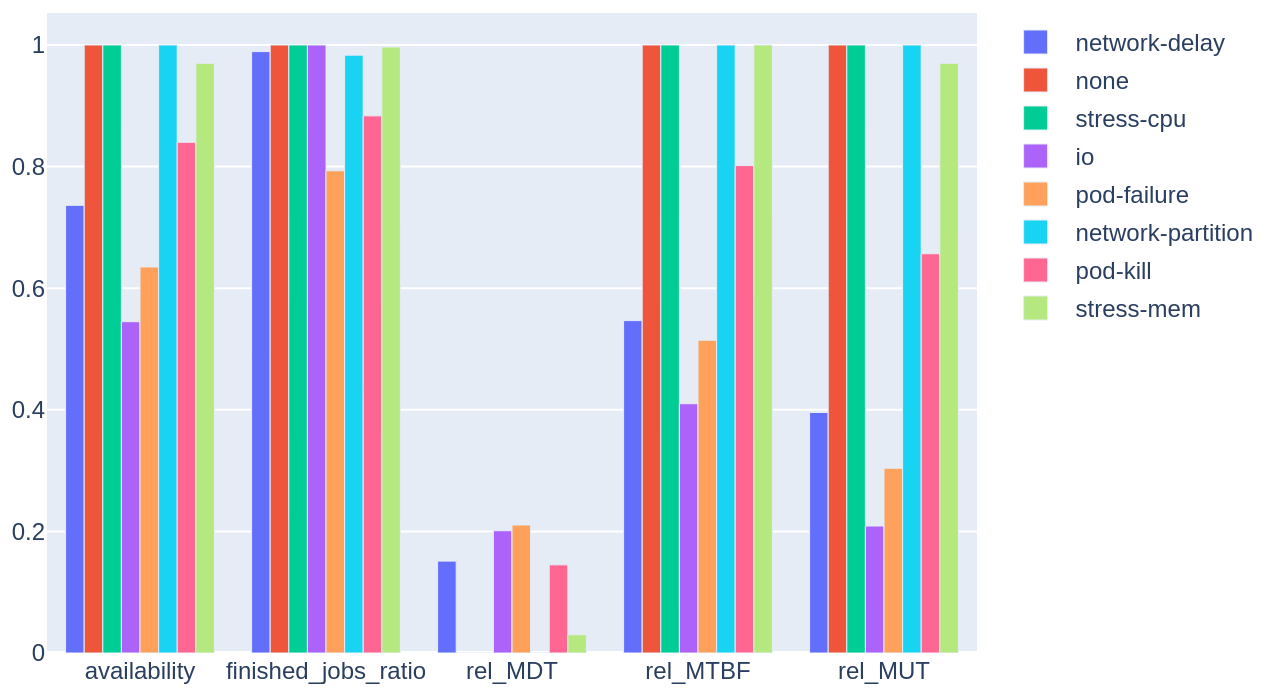
\includegraphics[width=140mm, keepaspectratio]{figures/baseline_grouped_barchart.png}
	\caption{Baseline Results}
	\label{fig:baseline_results}
\end{figure}

Looking at the results of the baseline measurements, one can notice several general correlations. It is not surprising, that the value of the \texttt{availability} greatly affects the value of the other three dependability metrics. A high \texttt{availability} means high \texttt{rel\_MUT}, while a lower value implies higher \texttt{rel\_MDT}. Generally, when the relative Mean Down Time is not zero, the results indicate more frequent faults (lower \texttt{rel\_MTBF} values).

As anticipated, the fault profile named "\texttt{none}" -- that does not inject any anomalies into the system -- delivered flawless metrics. The high value of \texttt{rel\_MTBF} can be counter-intuitive, however in a bounded time interval with no errors this is the right result, according to the formula described in Section \ref{background-dep-metrics-mean-values} (after normalization).

Applying the profiles "\texttt{stress-cpu}" and "\texttt{stress-mem} have only marginal effects on the metrics, that could a consequence of not enough injected simulated workload on the Pods. In this project, the task of fine-tuning of these chaos experiments remains open and is a good candidate for future work (see Section \ref{future-work}). However, for the sake of a thorough analysis, let us assume that the configuration of these chaos experiments lead to significant resource utilization anomalies (CPU and memory pressure). In Kubernetes, when the Pods on a given Node use up too much of the Node's resources, a couple of Pods get evicted from that Node to free up resources and are rescheduled on other Nodes, if possible \cite{KubernetesNodePressureEviction}. One might notice, that from the Pod's point of view, this prevention mechanism is similar to when the Pod simply gets deleted or killed due to an error. Of course, the user workload running on the Pod may experience performance issues before eviction, but in the end the application suffers from the same scenario: one of its component is stopped and restarted elsewhere in the cluster. Thus, if the system is prepared for sudden component fails and restarts, than it can also mitigate to some degree the effects of unexpected Node resource utilization growths.

Similarly the its two precedents, the fault profile named "\texttt{network-partition}" causes little falls in the metrics compared to the "\texttt{none}" profile. The root cause for this is probably the configuration of the chaos experiment. Its effects could be more severe, if the network partition occurred more frequently and affecting more Pods in the application namespace. This fine-tuning remains a possible next step for future work (see Section \ref{future-work}).

The fault profile named "\texttt{io}" produced the worst \texttt{availability} metric, however the \texttt{finished\_jobs\_ratio} value is the same as for the "\texttt{none}" profile. The reason for the lowest \texttt{availability} may well be in the mechanism how the backend component periodically checks if the database connection is still alive. Each time the backend performs a health check, it attempts to persist a test object and then sends a request to the database to query the newly created test data (as described in Section \ref{impl-backend-healthcheck}). One can notice that this is a synchronous mechanism. If writing to the database (which is stored on the disk) takes a long time because of the injected I/O delay, than the query that tries to retrieve the data can fail with a timeout error. Yet, during task executions, the application does not make an attempt to immediately check the persisted results, the communication remains asynchronous and the test framework only queries the jobs at the end of the measurements, after the load generation and fault injection is done.

The results of the fault profile "\texttt{network-delay}" show a similar characteristic as of the "\texttt{io}" -- significantly lower \texttt{availability} paired with little or no change in \texttt{finished\_jobs\_ratio} compared to the "\texttt{none}" profile. The reason for this is analogous as well. The steps of the health check implemented in the backend (see in Section \ref{impl-backend-healthcheck}) are using a synchronous communication model. For example, to test the connection between the backend and the worker components, a request is sent out from the backend and then it waits for a specific response. Due to the injected network delay, the health check can fail with a timeout error. However, as described above, during task executions, the communication follows an asynchronous pattern.

The "\texttt{pod-failure}" and "\texttt{pod-kill}" profiles introduce considerable changes in the metrics. As the results show, the "\texttt{pod-failure}" fault profile has more severe effects on the dependability than "\texttt{pod-kill}". This is not surprising, because "\texttt{pod-failure}" makes the affected Pods unavailable for a specific time, while "\texttt{pod-kill}" simply stops the Pods, enabling a ReplicaSet to immediately restart them (see Section \ref{test-impl-fault-profiles}). Both fault profiles can influence any component in the application. During the measurements, backend, database and message broker failures (or restarts) can degrade the \texttt{availability} of the application, whereas worker outages can generally lead to the loss of ongoing task executions, causing decline in \texttt{finished\_jobs\_ratio}. Of course, if all the worker components are down, the backend health check fails which further decreases the \texttt{availability}. The fact that the system handles the "\texttt{pod-kill}" fault profile better, supports the general notion why system developers prefer components that fail fast instead of long-lasting erroneous periods with undeterministic outcomes.

%\begin{itemize}
%	\item compare and try to reason about the results
%	\item as anticipated, the none profile has flawless metrics (MTBF is one because of the bounded time period of the measurement without error, MUT + MDT a little counter intuitive)
%	\item the stresschaos experiments do not have much effect - maybe the amount of the simulated workload wasn't enough -- future work to finetune
%	\item network partition has little effect - fine-tuning - future work
%	\item iochaos - worst availability - probably because of the DB connection test saves a test objects and then it tries to query it and it timeouts -- however, finished\_jobs\_ratio is not affected (the jobs are queried at the end of the measurements when the chaos objects are deleted)
%	\item network-delay - timeout errors can occur during the health check of the backend - during the checks, pseudo synchronous request-response pairs are used and round trip time can be long with the injected delay -- however, to send the jobs and results, plain async messaging is used, the components do not wait for response --> no timeout error can occur
%	\item pod-failure and pod-kill both have considerable effects on the metrics - pod-failure is more severe as a targeted Pod stays in faulty state during the whole intervals while the chaos is active - pod-kill deletes the pod, but it will be recreated immediately due to ReplicaSets -- the metrics show that this fail-fast behaviour is the more desirable scenario in distributed systems ----- both affect the finished\_jobs\_ratio due to job executing worker fails --> these get lost
%\end{itemize}















